\section{Μεθοδολογία υλοποίησης} \label{subsection:4-1-implementation-methodology}

Για την επίτευξη των στόχων που ορίστηκαν και την οργάνωση της απαιτούμενης εργασίας σε διαχειρίσιμα μέρη, χρησιμοποιήθηκαν διάφορα εργαλεία και μέθοδοι ανάπτυξης λογισμικού, όπως το σύστημα ελέγχου εκδόσεων (version control system) Git, η μέθοδος οργάνωσης Scrum και οι διαδικασίες ανάπτυξης DevOps. Τα εργαλεία αυτά είναι δοκιμασμένα και έχουν εδραιωθεί στη σύγχρονη ανάπτυξη λογισμικού.

Μέσα από την χρήση των παραπάνω εργαλείων επιτυγχάνεται η ομαλή συνεργασία στην ανάπτυξη του λογισμικού. Κάθε μέλος της ομάδας δύναται να εργαστεί ανεξάρτητα και χωρίς την ανάγκη διαρκούς επικοινωνίας με τα υπόλοιπα μέλη. Οι στόχοι είναι σαφώς ορισμένοι και χωρισμένοι σε διαχειρίσιμα μέρη, τα οποία δεν καταβάλλουν τα μέλη. Ταυτόχρονα, έχοντας ως έδρα καθιερωμένα πρότυπα ανάπτυξης, παρέχεται φορμαλισμός και έτοιμες μέθοδοι επίλυσης προβλημάτων, γεγονός που λειτουργεί καταλυτικά και βοηθά στην αποφυγή τελμάτων κατά τη συγγραφή του κώδικα.

Το Git\footnote{\url{https://git-scm.com/}} είναι δωρεάν λογισμικό ανοιχτού κώδικα, το οποίο επιτρέπει και επικουρεί την απρόσκοπτη ανάπτυξη λογισμικού από πολλαπλά μέλη μίας ομάδας, ταυτόχρονα και διανεμημένα. Αυτό το επιτυγχάνει ενσωματώνοντας ένα σύνολο από εργαλεία, τα οποία βοηθούν στη διαχείριση και στην ενσωμάτωση των διαφορετικών εκδόσεων του κώδικα που αναπτύσσει ξεχωριστά το κάθε μέλος της ομάδας. Υπάρχουν διάφορα μοντέλα χρήσης του Git και, πιο συγκεκριμένα, της δυνατότητας που παρέχει για δημιουργία, ανάπτυξη και ένωση (merge) κλαδιών (branches).

Για τους σκοπούς της παρούσας διπλωματικής χρησιμοποιήθηκε το μοντέλο GitHub flow\cite{4.1-github-flow}. Το μοντέλο αυτό ορίζει ότι κάθε προγραμματιστής ανοίγει ένα νέο branch για την ανάπτυξη ενός χαρακτηριστικού της εφαρμογής ή για τη διόρθωση ενός μέρους του κώδικα. Έπειτα, όταν η εργασία έχει ολοκληρωθεί, δημιουργείται ένα αίτημα ένωσης (pull request) με το βασικό κλαδί ανάπτυξης (develop) της εφαρμογής. Η εργασία υπόκειται σε αξιολόγηση από την υπόλοιπη ομάδα (review) και, όταν κριθεί ότι ικανοποιεί τις ανάγκες του έργου, το κλαδί ενώνεται με το develop. Όταν το develop φτάσει σε ικανό σημείο σταθερότητας και αλλαγών, γίνεται merge με το κλαδί παραγωγής (master). Από το κλαδί develop δημιουργούνται οι δοκιμαστικές εκδόσεις αιχμής της εφαρμογής, οι οποίες χρησιμοποιούνται κατά τον έλεγχο (staging versions), ενώ από το master δημιουργούνται οι τελικές της εκδόσεις, οι οποίες διανέμονται για χρήση στην παραγωγή (production versions).

Το Scrum είναι μία μέθοδος οργάνωσης, στην οποία ο επιμελητής του Scrum (Scrum master) διαχωρίζει τα ανεξάρτητα μέρη εργασίας (tasks) που πρέπει να υλοποιηθούν για την ολοκλήρωση των στόχων ενός project. Τα μέρη αυτά περιγράφονται αναλυτικά μαζί με τις απαιτήσεις τους και κατατίθενται σε μία λίστα εργασιών (backlog). Έπειτα, μέσα από συσκέψεις (meetings), επιλέγεται ένας αριθμός από task, τα οποία ορίζουν το επόμενο προγραμματιστικό κύκλο (Sprint). Κάθε task ανατίθεται σε κάποιο μέλος για υλοποίηση. Για το Sprint ορίζεται μία χρονική διάρκεια, στόχος της οποίας είναι η περάτωση όλων των task πριν τη λήξη της. Στο τέλος της προθεσμίας που ορίστηκε για το Sprint, τα μέλη της ομάδας αποτιμούν τα αποτελέσματα και ορίζουν το επόμενο Sprint. Η διαδικασία επαναλαμβάνεται έως ότου το έργο ολοκληρωθεί.

Λόγω του πολύ μικρού μεγέθους της ομάδας, το Scrum ακολουθήθηκε ελαστικά. Συγκεκριμένα, δεν ορίστηκε ένας συγκεκριμένος επιμελητής του board, αλλά κάθε μέλος της ομάδας φρόντιζε για τον ορισμό και την περιγραφή ενός μέρους των task. Τα Sprint δεν ήταν συνεχόμενα και δεν είχαν πάντα τον ίδιο χρόνο εκτέλεσης, αλλά προσαρμόζονταν ανάλογα με τις εκάστοτε ανάγκες και τον χρόνο των μελών. Για την οπτικοποίηση των task χρησιμοποιήθηκε κατά βάση η μέθοδος Kanban (που χρησιμοποιείται από το ίδιο το Scrum). Τα task χωρίστηκαν κατά κύριο λόγο στις παρακάτω λίστες:

\begin{itemize}
    \item "Αναμονής" (backlog), η οποία περιέχει task τα οποία δεν έχουν ακόμα εισαχθεί σε κάποιο sprint
    \item "Ενεργού Sprint" (sprint/todo), που περιλαμβάνει task τα οποία συμμετέχουν στο ενεργό (τρέχον) Sprint
    \item "Εκτέλεσης" (in progress/doing), η οποία περιλαμβάνει task για τα οποία έχει ξεκινήσει η ανάπτυξη από κάποιο μέλος της ομάδας
    \item "Ελέγχου και αξιολόγησης" (testing/code review), η οποία περιέχει task των οποίων η ανάπτυξη έχει ολοκληρωθεί και βρίσκονται στο στάδιο ελέγχου (testing) ή αναμονής σε pull request
    \item "Ολοκλήρωσης" (done), που περιλαμβάνει task τα οποία έχουν τελειώσει, δηλαδή των οποίων η ανάπτυξη έχει ολοκληρωθεί και το pull request έχει ενωθεί στο develop
\end{itemize}

Επίσης, ορίστηκαν στις λίστες οι μέγιστοι αριθμοί από task που μπορούν τα υπάρχουν σε κάθε χρονική στιγμή (π.χ. μέχρι τέσσερα task στη λίστα εκτέλεσης). Αυτό έγινε για ενθάρρυνση της ολοκλήρωσης των task από τα μέλη, σε αντίθεση με την εγκατάλειψή τους σε ημιτελή κατάσταση ανάπτυξης για την ανάληψη κάποιου νέου task.

Για την υλοποίηση του Scrum χρησιμοποιήθηκε η διαδικτυακή υπηρεσία Trello\footnote{\url{https://trello.com/}}, στιγμιότυπο της οποίας φαίνεται στο παρακάτω σχήμα:

\vspace{.25\baselineskip}

\begin{figure}[H]
    \centering
    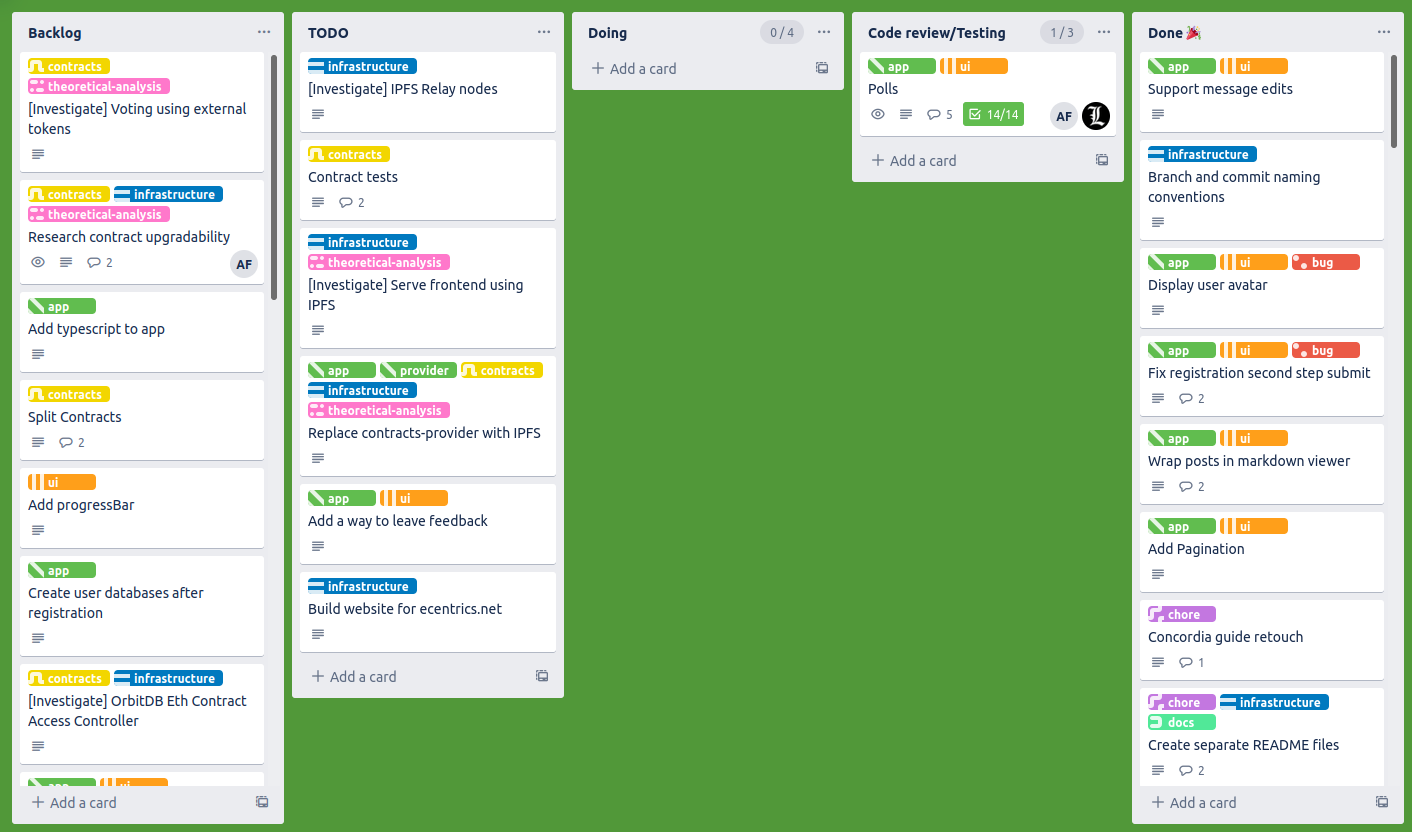
\includegraphics[width=\textwidth]{assets/figures/chapter-4/4.1.implementation-methodology-kanban}
    \caption{Στιγμιότυπο οθόνης της διαδικτυακής υπηρεσίας Trello}
    \label{figure:4.1.implementation-methodology-kanban}
\end{figure}

Κατά τη διαδικασία της ανάπτυξης του κώδικα, εφαρμόστηκαν επίσης οι τακτικές που ορίζονται από το DevOps σε ό,τι αφορά στο deployment των υπηρεσιών. Το DevOps ορίζει διάφορα εργαλεία που αποσκοπούν στην ταχεία, απρόσκοπτη και αυτοματοποιημένη ενσωμάτωση του κώδικα από το στάδιο της συγγραφής μέχρι την ολοκλήρωση και την εγκατάσταση. Τα εργαλεία που χρησιμοποιήθηκαν εδώ είναι:

\begin{itemize}
    \item Συνεχής έλεγχος (continuous testing)
    \item Συνεχής ολοκλήρωση (continuous integration)
    \item Συνεχής παράδοση (continuous delivery)
    \item Συνεχής εγκατάσταση (continuous deployment)
\end{itemize}

Για την υλοποίηση αυτών των τακτικών επιλέχθηκε μετά από εκτενή έρευνα η πλατφόρμα \hyperref[subsection:4-2-1-3-jenkins]{Jenkins}. Το Jenkins συνδυάστηκε με την πλατφόρμα εικονοποίησης \hyperref[subsection:4-2-1-2-docker]{Docker}, ώστε να ακολουθηθούν οι τελευταίες ενδεδειγμένες πρακτικές της βιομηχανίας. Έτσι, έγινε συγγραφή του αρχείου Jenkinsfile, το οποίο περιγράφει με κώδικα τη ροή εργασιών (pipeline) που πρέπει να ακολουθηθεί μετά από κάθε αλλαγή στον κώδικα. Η εκτέλεση του pipeline πραγματοποιείται αυτόματα από το Jenkins.

Η ροή εργασιών αποτελείται από στάδια και βήματα τα οποία φαίνονται στο σχήμα \ref{figure:4.1.implementation-methodology-jenkins-pipeline}:

\begin{enumerate}
    \item Αρχικά εκτελείται το βήμα "Version", το οποίο συλλέγει στοιχεία σχετικά με την εκτέλεση του pipeline, όπως το κλαδί του κώδικα που πυροδότησε τη ροή και τα πακέτα λογισμικού που περιλαμβάνονται στο git repository και περιέχουν αλλαγές.
    \item Έπειτα εκτελείται το στάδιο "TEST", το οποίο περιέχει δύο βήματα που εκτελούνται παράλληλα και πραγματοποιούν έλεγχο του κώδικα των πακέτων.
    \item Αν το κλαδί πυροδότησης είναι ένα feature branch η ροή σταματά εδώ, ενώ αν πρόκειται για ένα από τα βασικά κλαδιά (master ή develop), τότε η ροή συνεχίζει με το στάδιο "BUILD", στο οποίο εκτελούνται παράλληλα τα βήματα που χτίζουν τα docker image όσων πακέτων περιέχουν αλλαγές.
    \item Στο στάδιο "PUBLISH", αν το κλαδί πυροδότησης είναι το κύριο κλαδί παραγωγής (master), τότε εκτελούνται παράλληλα βήματα τα οποία δημοσιεύουν τα docker image που δημιουργήθηκαν στο αποθετήριο Docker Hub.
    \item Τέλος, εκτελείται το στάδιο "DEPLOY", κατά το οποίο πραγματοποιείται η εγκατάσταση των υπηρεσιών στο ανάλογο περιβάλλον (staging για το κλαδί develop και production για το κλαδί master).
\end{enumerate}

\begin{figure}[H]
    \centering
    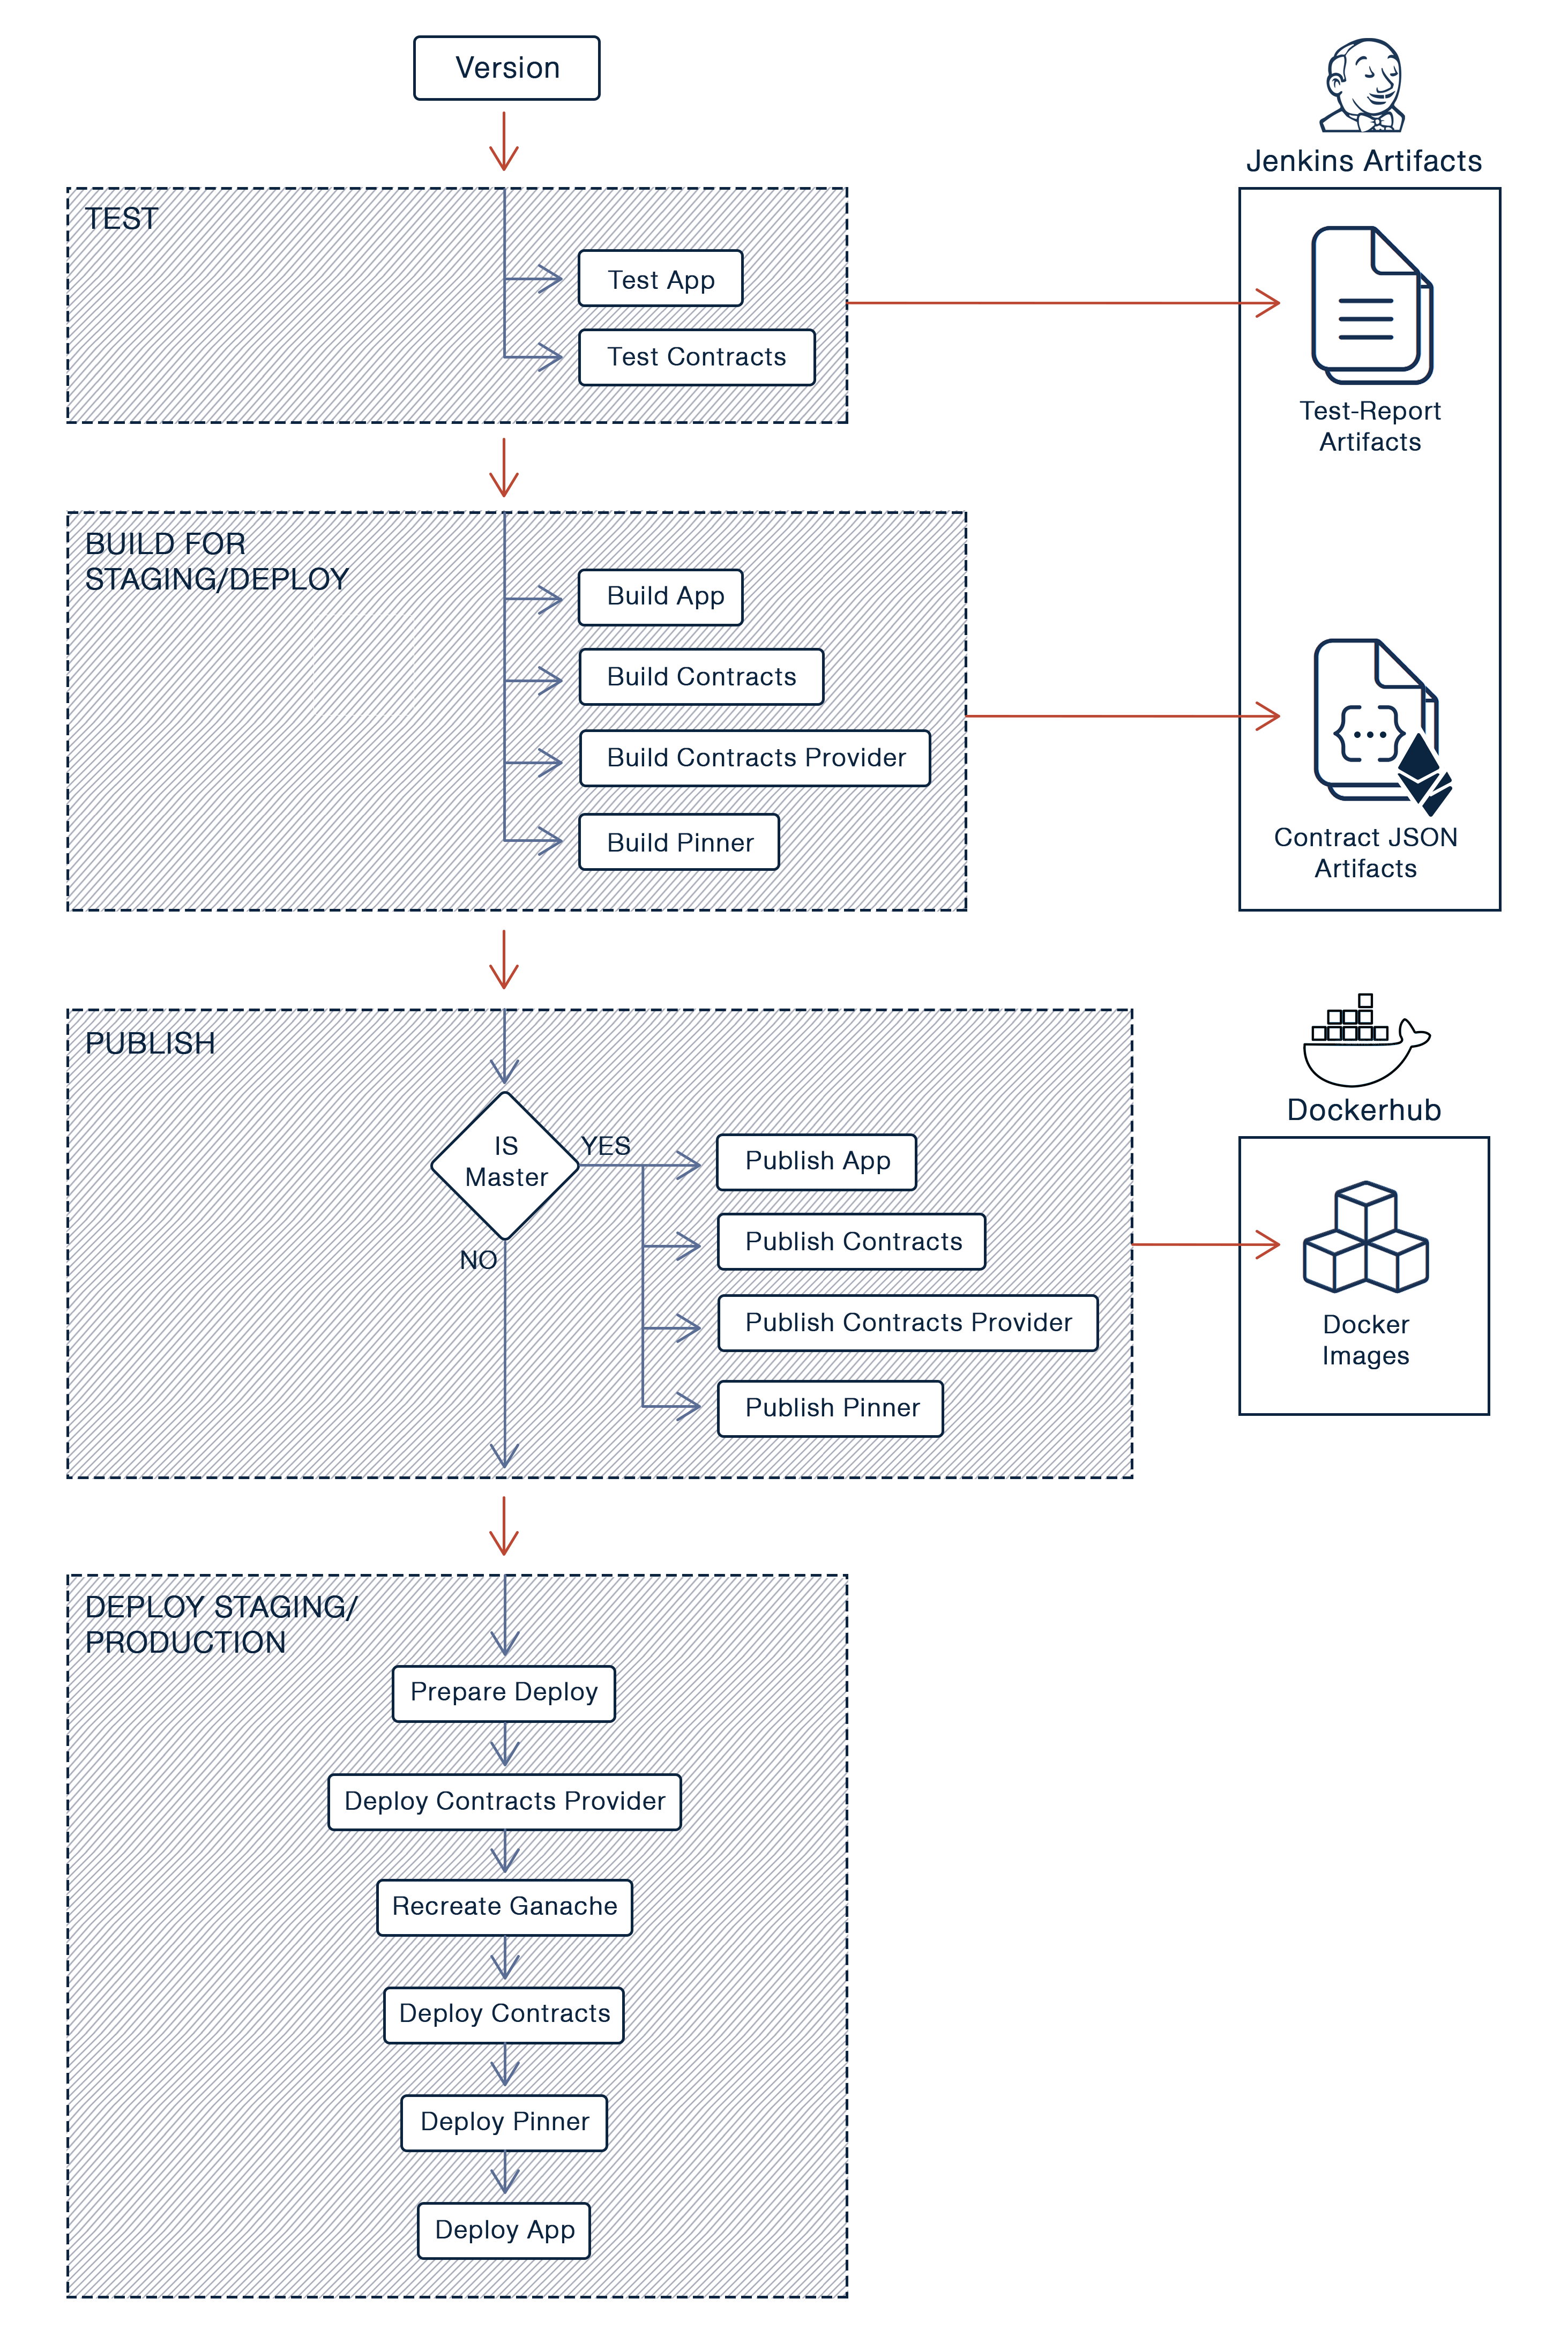
\includegraphics[width=.9\textwidth]{assets/figures/chapter-4/4.1.implementation-methodology-jenkins-pipeline}
    \caption{Διάγραμμα ροής εργασιών Jenkins}
    \label{figure:4.1.implementation-methodology-jenkins-pipeline}
\end{figure}

\vspace{\baselineskip}

Με τη χρήση του Jenkins αυτοματοποιείται με μεγάλη ευκολία ένα σημαντικό μέρος των διαδικασιών ανάπτυξης και δημοσίευσης του κώδικα. Με τη χρήση της συγκεκριμένης ροής εργασιών εξασφαλίζεται ότι σε κάθε αλλαγή, ασχέτως του κλαδιού ανάπτυξης, ο κώδικας ελέγχεται και τα αποτελέσματα των test είναι αποθηκευμένα και διαθέσιμα για ανάλυση. Ακόμα, για το κλαδί develop, αυτοματοποιείται η ολοκλήρωση των πακέτων και η εγκατάστασή τους σε περιβάλλον δοκιμής (staging), γεγονός που διευκολύνει σημαντικά τις συλλογικές δοκιμές από την ομάδα σε διαφορετικά περιβάλλοντα χρήσης (browsers). Τέλος, για το κλαδί master, αυτοματοποιείται η διαδικασία δημοσίευσης των docker image, μηδενίζοντας έτσι τον χρόνο που πρέπει να καταβάλλουν τα μέλη της ομάδας σε αυτό.
